\documentclass[10pt,openright]{report}

\usepackage[utf8]{inputenc}
\usepackage[swedish]{babel}
\usepackage{color}
\usepackage[activate={true,nocompatibility},final,tracking=true,kerning=true,spacing=true,factor=1100,stretch=10,shrink=10]{microtype}
\usepackage[a4paper,twoside,twocolumn,inner=2.2cm,outer=1.9cm,columnsep=0.9cm,top=2cm,bottom=2cm]{geometry}
\usepackage{fancyhdr}
\usepackage[scaled]{helvet}
\renewcommand\familydefault{\sfdefault}
\usepackage[T1]{fontenc}
\usepackage{tabularx}
\usepackage{enumitem}  \setlist{nolistsep}
\usepackage{graphicx}

\pagestyle{fancy}
\lhead{}
\chead{}
\rhead{}
\cfoot{}
\fancyfoot[LE,RO]{\thepage}
\renewcommand{\headrulewidth}{0pt}

%% This fixes page numbering on chapter head pages
\fancypagestyle{plain}{
  \fancyhf{}
  \fancyfoot[LE,RO]{\thepage}
  \renewcommand{\headrulewidth}{0pt}}

\renewcommand\thepart{\Alph{part}}

\usepackage[raggedright]{titlesec}
\titlespacing{\chapter}{0pt}{1cm}{1cm}
\titleformat{\chapter}[hang]{\Huge\bfseries}{\fcolorbox{black}{black}{\color{white}\,\thepart\thechapter\,}~~}{0pt}{\Huge\bfseries}
\titleformat{\part}[hang]{\Huge\bfseries}{\fcolorbox{black}{black}{\color{white}\,\thepart\,}~~}{0pt}{\Huge\bfseries}

\renewcommand{\thesection}{\thepart\thechapter.\arabic{section}}

%%% Common macros
\newcommand{\enhet}[1]{\SI{}{#1}}
\newcommand{\vbokstav}[1]{$#1$}

\usepackage{siunitx}
%%\sisetup{output-decimal-marker = {,}}
\sisetup{locale=FR}

\begin{document}

\setlength{\parindent}{0pt}
\setlength{\parskip}{1ex plus 0.5ex minus 0.5ex}



\setcounter{part}{19}
\setcounter{chapter}{0}
\part{Teknik}

\chapter{Ellära}
\section{Ström}

Elektrisk ström består av elektroner, som
förflyttar sig genom en ledning. Elektronerna
är bärare av elektriska laddningar. Ju fler
elektroner, desto högre ström. Elektronerna
förflyttar sig i motsatt riktning mot strömmen.
Strömstyrka mäts med enheten \emph{Ampere,}
förkortat \enhet{A}.

%%% Bild strömriktning -- elektroners riktning

\[
\begin{array}{rclcl}
\SI{1}{A}  &=& \SI{1000}{mA} \\
\SI{1}{mA} &=& \SI{0.001}{A} \\
\SI{1}{\micro A} &=& \SI{0.001}{mA} &=& \SI{0.000001}{A}
\end{array}
\]

Som symbol för ström används \vbokstav{I}.

\section{Spänning}

För att få elektroner att förflytta sig gen\-om
en ledning behövs en drivande kraft. Denna
kraft kallas den el\-ek\-tro\-mo\-to\-ris\-ka kraften
eller spänning. Spänningen kan jämföras
med trycket i en vattenledning. Ju högre
tryck i ledningen, desto mer vatten kommer
det ur kranen. Ju högre spänning vi har, desto
mer ström flyter det genom en ledning.
Spänning mäts i enheten \emph{Volt,} förkortat \enhet{V}.

\[
\begin{array}{rcl}
\SI{1}{kV} &=& \SI{1000}{V} \\
\SI{1}{mV} &=& \SI{0.001}{V} \\
\SI{1}{\micro V} &=& \SI{0.001}{mV}
\end{array}
\]

Som symbol för spänning används \vbokstav{U}.

\section{Resistans -- motstånd}

Hur mycket ström det flyter i en ledning
vid en given spänning beror på de egenskaper
som ledaren har, d.v.s. hur lätt strömmen
flyter. En tunn ledning gör det svårare för
strömmen att flyta. Ledaren erbjuder större
motstånd än en grov ledare. Resistans mäts i enheten Ohm -- \enhet{\Omega}
(grekiska bokstaven omega).

\[
\begin{array}{rclcl}
\SI{1}{k\Omega} &=& \SI{1000}{\Omega} \\
\SI{1}{M\Omega} &=& \SI{1000}{k\Omega} &=& \SI{1000000}{\Omega}
\end{array}
\]

Som symbol för resistans används \vbokstav{R}.

\section{Grundenheter}

Enheterna \enhet{A}, \enhet{V} och \enhet{\Omega} är grundenheter.

\subsection{Definition}

Definitionen för dessa grundenheter är att
vid spänningen $U = \SI{1}{Volt}$ och resistansen
$R = \SI{1}{Ohm}$, kommer det att flyta en ström
$I = \SI{1}{Ampere}$.

%%% Bild: spänning över och ström genom resistor

\section{Ohms lag}

Ohms lag är en grundformel, som kan
utvecklas och användas till att räkna ut det
mesta inom elektronik. Man använder symbolerna: \vbokstav{I}, \vbokstav{U} och \vbokstav{R}.

\[
\begin{array}{rclcl}
  I &=& \frac{U}{R} &\quad& \text{Ampere} \\
  \\
  U &=& R \cdot I &\quad& \text{Volt} \\
  \\
  R &=& \frac{U}{I} &\quad& \text{Ohm}
\end{array}
\]

För att lättare komma ihåg sambandet, kan man förenkla det hela genom nedanstående
figurer. Täck över den symbol du vill beräkna.

%%\smalltikz{\tikz\node[Formeldreieck]{$\dfrac{U}{R\cdot I}$};}{Formeltriangel för ohms lag.}{fig:ohmslag}

\smalltikz{
\begin{tikzpicture}%%BASE
  \path (0,0) node [regular polygon,regular polygon sides=3,draw,minimum size=2cm] {};
%%  \filldraw[fill=gray] (0,0.133) -- (0,-.499) -- (.86,-.499) -- (.5,0.133) -- cycle;
  \draw (-0.499,0.133) |- (0.499,0.133);
  \path (0,0.7) node [anchor=north] {$U$};
  \path (-0.3,0.05) node [anchor=north] {$R$};
  \path (0.3,0.05) node [anchor=north] {$I$};
  \draw (0,0.133) -- (0,-0.5);
  \path (0,0) node [anchor=north,fill=white] {$\cdot$};
  \vspace{1ex}
%%  \node[align=center,anchor=north] at (0,-1) { };
  \node[align=center,anchor=north,text=white] at (0,-1) {$R=\dfrac{U}{I}$};
\end{tikzpicture}
\hspace{1ex}
\begin{tikzpicture}%%U=RI
  \path (0,0) node [regular polygon,regular polygon sides=3,draw,minimum size=2cm] {};
  \filldraw[fill=gray] (-.5,0.133) -- (0,1) -- (.5,0.133) -- cycle;
  \draw (-0.499,0.133) |- (0.499,0.133);
  \path (0,0.7) node [anchor=north] {$U$};
  \path (-0.3,0.05) node [anchor=north] {$R$};
  \path (0.3,0.05) node [anchor=north] {$I$};
  \draw (0,0.133) -- (0,-0.5);
  \path (0,0) node [anchor=north,fill=white] {$\cdot$};
  \node[align=center,anchor=north,text=white] at (0,-1) {$R=\dfrac{U}{I}$};
  \node[align=center,anchor=north] at (0,-1.25) {$U=R\cdot I$};
\end{tikzpicture}
\hspace{1ex}
\begin{tikzpicture}%%I=U/R
  \path (0,0) node [regular polygon,regular polygon sides=3,draw,minimum size=2cm] {};
  \filldraw[fill=gray] (0,0.133) -- (0,-.499) -- (.86,-.499) -- (.5,0.133) -- cycle;
  \draw (-0.499,0.133) |- (0.499,0.133);
  \path (0,0.7) node [anchor=north] {$U$};
  \path (-0.3,0.05) node [anchor=north] {$R$};
  \path (0.3,0.05) node [anchor=north] {$I$};
  \draw (0,0.133) -- (0,-0.5);
%%  \path (0,0) node [anchor=north,fill=white] {$\cdot$};
  \node[align=center,anchor=north] at (0,-1) {$I=\dfrac{U}{R}$};
\end{tikzpicture}
\hspace{1ex}
\begin{tikzpicture}%%R=U/I
  \path (0,0) node [regular polygon,regular polygon sides=3,draw,minimum size=2cm] {};
  \filldraw[fill=gray] (0,0.133) -- (0,-.499) -- (-.86,-.499) -- (-.5,0.133) -- cycle;
  \draw (-0.499,0.133) |- (0.499,0.133);
  \path (0,0.7) node [anchor=north] {$U$};
  \path (-0.3,0.05) node [anchor=north] {$R$};
  \path (0.3,0.05) node [anchor=north] {$I$};
  \draw (0,0.133) -- (0,-0.5);
%%  \path (0,0) node [anchor=north,fill=white] {$\cdot$};
  \node[align=center,anchor=north] at (0,-1) {$R=\dfrac{U}{I}$};
\end{tikzpicture}
}{Formeltriangel för ohms lag.}{fig:ohmslag}

%% \begin{tikzpicture}
%%   \draw (0,0) -- (1,1.5);
%%   \draw (1,1.5) -- (2,0);
%%   \draw (0,0) -- (2,0);
%%   \draw (0.45,0.66) -- (1.55,0.66);
%%   \draw (1,0) -- (1,0.66);
%%   \node at (1,1) {U};
%%   \node at (0.66,0.25) {R};
%%   \node at (1.25,0.25) {I};
%% \end{tikzpicture}


\chapter{Komponenter -- egenskaper}
\input{blabok/t02.tex}

\chapter{Kretsar}
\input{blabok/t03.tex}

\chapter{Radiosändaren}
\input{blabok/t04.tex}

\chapter{Radiomottagaren}
\input{blabok/t05.tex}

\chapter{Kablar och antenner}
\input{blabok/t06.tex}

\chapter{Vågutbredning}
\input{blabok/t07.tex}

\chapter{Mätning, mätinstrument}
\input{blabok/t08.tex}

\chapter{Störningar}
\input{blabok/t09.tex}

\chapter{Elsäkerhet}
\input{blabok/t10.tex}


\setcounter{part}{17}
\setcounter{chapter}{0}
\part{Reglemente}

\chapter{Fonetiska alfabetet}
Varje kapitel avslutas med två rutor, ”Kom ihåg!” och ”Lär dig...”.
Dessa rutor ska enbart ses som en samman- fattning av det viktigaste i
respektive kapitel. Ett antal övningsfrågor till kapitlen och facit
finns längre bak i boken. Ytterligare övningsfrågor finns på SSA:s
webbplats www.ssa.se

Det totala innehållet i kapitlen utgör underlag för provfrågorna för
amatörradiocertifikat/licens. Prov avläggs för en av SSA auktoriserad
<provförrättare.

\section{Bokstavering}

För att underlätta mottagning av anropssignaler, obekanta ord,
svårförståeliga namn eller förkortningar, använder man sig av
bokstavering. Bokstavering innebär, att varje enskild bokstav har fått
ett personnamn. Personnamnen har valts ut med hänsyn till hur lätta de
är att ur- och särskilja i till exempel störd miljö.

\subsection{Svenska bokstaveringsalfabetet}

\begin{table}[h]
  \begin{tabular}{ll|ll}
    A & Adam   & P & Petter  \\
    B & Bertil & Q & Quintus \\
    C & Cesar  & R & Rudolf  \\
    D & David  & S & Sigurd  \\
    E & Erik   & T & Tore    \\
    F & Filip  & U & Urban   \\
    G & Gustav & V & Viktor  \\
    H & Helge  & W & Wilhelm \\
    I & Ivar   & X & Xerxes  \\
    J & Johan  & Y & Yngve   \\
    K & Kalle  & Z & Zäta    \\
    L & Ludvig & Å & Åke     \\
    M & Martin & Ä & Ärlig   \\
    N & Niklas & Ö & Östen   \\
    O & Olof   &   &         \\
  \end{tabular}
  \caption{Svenska bokstaveringsalfabetet}
  \label{tab:sv-bokstavering}
\end{table}

Om man alltid använder samma namn, så kan man i en störd miljö gissa
sig till vilken bokstav som menas. Vid bokstavering uttalas bokstaven
A som ADAM, bokstaven B som BERTIL och så vidare.

Det finns även ett internationellt boksta- veringsalfabet (på
engelska). Det används på motsvarande sätt som det svenska
bokstaveringsalfabetet. Internationellt är det mycket viktigt att inte
hitta på andra engelska ord eller namn, eftersom motstationen kanske
inte kan engelska.

\section{Internationella bokstaveringsalfabetet}

\begin{table}[h]
  \begin{tabular}{ll|ll}
    A & Alfa     & P & Papa  \\
    B & Bravo    & Q & Quebec\\
    C & Charlie  & R & Romeo\\
    D & Delta    & S & Sierra\\
    E & Echo     & T & Tango\\
    F & Foxtrot  & U & Uniform\\
    G & Golf     & V & Victor\\
    H & Hotel    & W & Whiskey \\
    I & India    & X & X-Ray\\
    J & Juliet   & Y & Yankee\\
    K & Kilo     & Z & Zulu\\
    L & Lima     & Å & Alfa Alpha\\
    M & Mike     & Ä & Alfa Echo\\
    N & November & Ö & Oscar Echo\\
    O & Oscar    & & \\
  \end{tabular}
  \caption{Internationella bokstaveringsalfabetet}
  \label{tab:int-bokstavering}
\end{table}



\vspace{1em} \hrule \vspace{1em}

\emph{Kom ihåg:}


\begin{itemize}
\item En korrekt bokstavering underlättar all radiokommunikation
\end{itemize}

\emph{Lär dig:}

\begin{itemize}
\item Bokstaveringsalfabetena som du måste kunna utantill!
\end{itemize}


\chapter{Q-koden}
\section{Q-koden}

Q-koden är internationell och har därför fördelen att den kan försås
av alla oberoende av vilket språk som använde.

Förkortningar och Q-koder var ursprungligen tänkta att användas vid
morsetelegrafering för att vinna tid. Numera används Q-koden vit
telegrafi, telefoni och vid digitala trafiksätt.

Q-koden består av bokstaven Q följd av ytterligare två bokstäver till
exempel QSL som betyder ``Jag kvitterar''.

Samma Q-förkortning kan användas som fråga: ``QSL?'' som betyder ``Kan
du ge mig kvittens?''

Andra Q-förkortningar kan användas tillsammans med t.ex. ett
klockslag, en ort, en frekvens m.m.

Ett klockslag:

\begin{itemize}
  \item QRX? -- När anropar du mig igen?
  \item QRX 2048 UTC -- Jag anropar dig igen klockan 20:48 UTC
\end{itemize}

En ort:

\begin{itemize}
\item QTH? -- Vilken är din geografiska position?
\item QTH KARLSBORG -- Min geografiska position är Karlsborg.
\end{itemize}

\scriptsize
\begin{table}[h]
  \begin{tabular}{ll}
    Q-kod & Betydelse som fråga och som svar\\ \hline

    QRK?  & Vilken uppfattbarhet har mina signaler?\\
    QRK   & Uppfattbarh. hos dina (eller *:s signaler) är:\\
          & 1. Dålig\\
          & 2. Bristfällig\\
          & 3. Ganska god\\
          & 4. God\\
          & 5. Utmärkt\\ \hline

    QRM?  & Är min sändning störd av annan station?\\
    QRM   & Störningarna på din signal är:\\
          & 1. Obefintliga\\
          & 2. Svaga\\
          & 3. Måttliga\\
          & 4. Starka\\
          & 5. Mycket starka\\ \hline

    QRN?  & Besväras du av atmosfäriska störningar?\\
    QRN   & Atmosfäriska störningar är:\\
          & 1. Obefintliga\\
          & 2. Svaga\\
          & 3. Måttliga\\
          & 4. Starka\\
          & 5. Mycket starka\\ \hline

    QRO? & Ska jag öka sändareffekten?\\
    QRO  & Öka sändareffekten \\ \hline

    QRP? & Ska jag minska sändareffekten? \\
    QRP  & Minska sändareffekten \\ \hline

    QRS? & Skall jag minska sändningstakten?\\
    QRS  & Minska sändningstakten \\ \hline

    QRQ? & Skall jag öka sändningstakten?\\
    QRQ  & Öka sändningstakten\\ \hline

    QRT? & Skall jag avbryta sändningen?\\
    QRT  & Avbryt sändningen \\ \hline

    QRV? & Är du redo?\\
    QRV  & Jag är redo\\ \hline

    QRX? & När anropar du mig igen?\\
    QRX  & Jag anropar dig igen kl ... (på ... MHz/kHz)\\ \hline

    QRZ? & Vem anropar mig?\\
    QRZ  & Du anropas av ... (på ... kHz/MHz)\\ \hline

    QSB? & Varierar min signalstyrka?\\
    QSB  & Din signalstyrka varierar\\ \hline

    QSL? & Kan du ge mig kvittens?\\
    QSL  & Jag kvitterar\\ \hline

    QSO? & Kan du få förbindelse med ...?\\
    QSO  & Jag kan få förbindelse med ...\\ \hline

    QSY? & Ska jag gå över till annan frekvens?\\
    QSY  & Jag byter frekvens till ... kHz/MHz\\ \hline

    QTH? & Vilken är din geografiska position?\\
    QTH  & Min geografiska position är ...\\ \hline
  \end{tabular}
  \caption{Q-koden}
  \label{tab:q-koden}
\end{table}
\normalsize

\vspace{1em} \hrule \vspace{1em}

\noindent\emph{Kom ihåg:}

\begin{itemize}
\item För att kunna betrakta dig som sändaramatör måste du kunna de allra
vanligaste Q-förkortningarna.

\item Q-förkortningarna används både på telegrafi och telefoni och i digital
trafik.
\end{itemize}

\noindent\emph{Lär dig:}

\begin{itemize}
\item De ovanstående Q-förkortningarna ska du kunna
utantill.

\item Var mycket uppmärksam på om Q-förkortningen åtföljs av ett
frågetecken eller inte.
\end{itemize}


\chapter{Amatörradioförkortningar}
Utöver Q-förkortningarna förekommer även internationella
amatörradioförkortningar, s.k. trafikförkortningar.

De flesta trafikförkortningarna bygger på engelska uttryck och används
framför allt vid telegrafi och digitala trafiksätt. Här följer ett
urval av de vanligaste förkortningarna.

\begin{table}[h]
  \begin{tabular}{lll}
    Förk. & Engelsk bet. & Svensk bet.\\
    BK & Break & Bryt\\
    & Signal used to interrupt a & Sänds för att avbryta\\
    & transmission in progress  & motstationens sändning\\
    CQ & General call to all stations & Allmänt anrop\\
    CW & Continuous wave & Telegrafi\\
    DE & From & Från\\
    & Separates the callsign      & Används vid telegrafi \\
    & of the station called from  & och digitala trafiksätt\\
    & that of the calling station & vid identifiering mellan\\
    &                             & motstationens och din egen\\
    &                             & anropssignal\\
    K & Invtation to send & Kom, jag lyssnar\\
    MSG & Message & Meddelande\\
    PSE & Please & Var vänlig och ...\\
    R & Received & Mottaget\\
    RST & Report system & Rapportsystem\\
    & R = Readability & R = Läsbarhet\\
    & S = Signal strength & S = Signalstyrka\\
    & T = Tone report & T = Tonkvalitet\\
    RX & Receiver & Radiomottagare\\
    TX & Transmitter & Radiosändare\\
    UR & Your & Din\\
  \end{tabular}
  \caption{Trafikförkortningar}
  \label{tab:trafikforkortningar}
\end{table}

\emph{Kom ihåg:}

För att kunna betrakta dig som sändaramatör måste du kunna de allra
vanligaste trafikförkortningarna.

Trafikförkortningarna används mest på telegrafi och digitala
trafiksätt.

\emph{Lär dig:}

Ovanstående trafikförkortningar som du måste kunna utantill.


\chapter{Internationella nödsignaler}
\section{Bestämmelser för nödtrafik}



\paragraph{Nödtrafik} \hfill \\

Trafik för att förebygga eller reducera ytterligare
skadeverkningar vid uppenbar risk för allvarlig person- eller
egendomsskada, eller då någon är svårt skadad eller i livsfara.

\paragraph{Nöd bryter lag} \hfill \\

Ingen bestämmelse i reglementet får utgöra hinder för en landstation
att under utomordentliga förhållanden begagna sig av alla till buds
stående medel för att bringa hjälp åt en nödställd rörlig station.


\paragraph{Nödsignaler vid sjö- och luftradiotrafik} \hfill \\

På telefoni utgörs nödsignalen av ordet MAYDAY (uttalas som det
franska ordet m'aider [mädé] och inte som [mäjdäj]).

Denna nödsignal tillkännager att ett fartyg, luftfartyg eller
färdmedel av annat slag hotas av allvarlig och överhängande fara och
begär omedelbar hjälp.

\paragraph{Internationella nödfrekvenser} \hfill \\

Utsändning av nödsignaler på telefoni på VHF-banden sker i första hand
på frekvenserna \SI{121,5}{MHz} för flyg och på kanal 16 VHF Marin på
\SI{156,8}{MHz}. Tidigare har kanal 16 på privatradiobandet också
använts för nödsignalering men har i dag ingen officiell status.

Utsändning av nödsignaler på HF (kortvåg) kan ske på vilken frekvens
som helst. 


\section{Åtgärder då nödsignaler uppfattas}

När man uppfattar ett nödanrop så är det viktigt att först vänta och
höra om någon annan station svarar.

\begin{tabularx}{\columnwidth}{lX}
  \textbf{Avbryt} & Avbryt egen lyssning \\\hline
  \textbf{Lyssna} & Avlyssna och skriv ner nödmeddelandet, position,
  frekvens med mera som är av vikt. \\\hline
  \textbf{Larma} & Kvitteras inte nödsignalen från mark- eller
  kustradiostation, ring 112, invänta telefonistsvar och begär
  Flygräddning eller Sjöräddning och meddela dina iakttagelser\\\hline
\end{tabularx}

Tänk på följande om du får kontakt med en nödställd:

\begin{tabularx}{\columnwidth}{lX}
  \textbf{Var?} & Var finns olycksplatsen? Position? \\ \hline
  \textbf{Vad?} & Vad har inträffat? \\ \hline
  \textbf{Vem?} & Vem är det som anropar? (Anropssignal, namn på
  fartyg) \\ \hline
  \textbf{Hur?} & Vad behöver den nödställde för hjälp? (Ambulans,
  medicin, brandkår, sjöräddning, flygräddning)\\ \hline
  \textbf{När?} & Notera tidpunkt och frekvens när du uppfattade
  nödmeddelandet\\ 
\end{tabularx}

\section{Nödsignalering på amatörradiobanden}

På amatörradiofrekvenser kan signalen \textbf{CQ EMERGENCY}
(nödmeddelande) förekomma som nödsignal vid nödsituationer på land när
allvarlig och överhängande fara hotar människoliv.

Nödsignalen bör åtföljas av ett nödmeddelande där det anges nödlägets
art, plats samt vilken hjälp som behövs.

Detta är dock INTE en officiellt erkänd nödsignal.

\textit{Vid nödanrop, följ åtgärdslistan i tillämpliga delar enligt
  föregående sida.} \\[1em] \hrule

\emph{Kom ihåg:}

\begin{itemize}
\item MAYDAY
\item CQ EMERGENCY
\item När du uppfattar ett nödanrop så ädet viktigt att först vänta och
  lyssna om någon annan station svarar
  \itemÅtgärder: Avbryt, Lyssna, Larma 112
\end{itemize}

\emph{Lär dig:}

\begin{itemize}
\item  Vad du skall göra om du uppfattar ett nödanrop
\end{itemize}


\chapter{Anropssignler}
\section{Anropssignal}

Innehavare av ett amatörradiocertifikan eller amatörradiotillstånd ska
ha egen anropssignal. Enligt det internationella radioreglementet ska
anropssignalen för an amatörradiostation inledas med ett \emph{prefix}
som i princip är en landskod vilken består av en eller två bokstäver.
En av de två bokstäverna kan bytas mot en siffra.

Efter prefixet ska det komma en \emph{siffra} och därefter avslutas
signalen med ett \emph{suffix} som är person eööer stationskoden.

Exempel på anropssignaler: SM4UEI, SA0LAT, SK0UX.

Där SM är prefixet för sverige i den äldre standarden när televerket
utdelade signaler, 4 är distriktssiffran för dalarna och värmland, UEI
är den personliga anropssignalen.

För SA0LAT är det SA som är prefixet för sverige, 0 är
distriktssiffran för stockholmsområdet och LAT är den personliga
anropssignalen.

I den sista, SK0UX, så är landsprefixet SK för sverige, 0 för
stockholmsområdet och UX är stationskoden. Denna signal är en
radioklubbsignal, serien SK används bara för detta.

\section{Sveriges distrikt}

Sverige delas in i ett antal geografiska distrikt. Dessa distrikt ger
siffran mellan prefix och suffix i en anropssignal. Normalt används
den distriktsiffra där radioamatören är folkbokförd.

\begin{tabularx}{\columnwidth}{lX}
  \textbf{Distrikt} & \textbf{Område}\\ \hline
  0 & Stockholm\\
  1 & Gotland\\
  2 & Västerbotten, Norrbotten\\
  3 & Gävleborg, Västernorrland, Jämtland\\
  4 & Dalarna, Värmland\\
  5 & Uppsala, Södermanland, Östergötland, Västmanland\\
  6 & Halland, Västra Götaland\\
  7 & Jönköping, Kronoberg, Kalmar, Blekinge, Skåne\\
\end{tabularx}

\begin{figure}
  \centering
  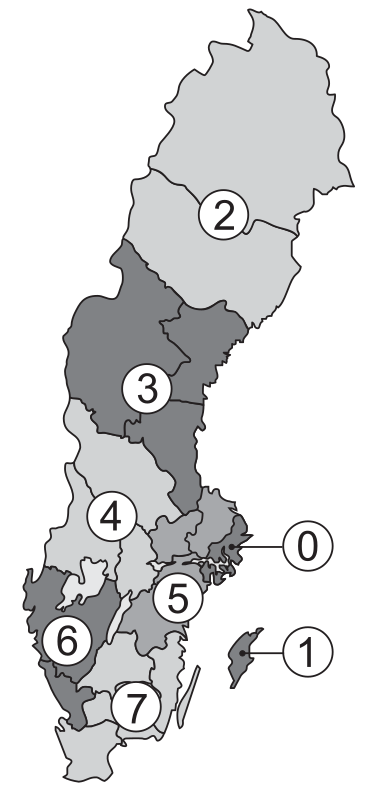
\includegraphics[width=.5\columnwidth]{blabok/pictures/R5-1.png}
\end{figure}

%Layout
\newpage

\section{Svenska prefix}

I Sverige finns flera olika prefix som kan användas. Nya radioamatörer
får alltid en signal med prefix SA. Äldre amatörer som avlade sitt
prov på den tiden televerket höll i provförrättningen fick signaler
med prefix SM. Dessa är de vanligaste prefixen som används.

Radioklubbar kan få signaler med prefix SA eller SK. Militära
amatörradiostationer och FRO (Frivilliga Radioorganisationen) får
signaler med prefixet SL.

För specialsignaler kan om det finns särskilda skäl för detta, t.ex.
för radiotävlingar och liknande ändamål, specialsignaler tilldelas.
Dessa tilldelas i någon av serierna 7S, 8S, SA, SB, SC, SD, SE, SF,
SG, SH, SI, SJ, SK, SL och SM.

%Layout
\newpage

\section{Anropssignaler}

\paragraph{Amatörradiosignalens utformning} \hfill \\

Tidigare har myndigheterna krävt att anropssignalen ska visa så
detaljerat som möjligt varifrån utsändningen äger rum. Detta krav
finns inte längre.

Praxis är numera att:

\begin{itemize}
\item Vid sändning från din ordinaria bostad
  (folkbokföringsadressen) används din vanliga anropssignal
  exempelvis SA0LAT.
\item Vi sändning från annan plats, t.ex. sommarbostad eller
  motsvarande visas detta genom att lägga till distriktsiffran där
  du befinner dig för tillfället, till exempel: SM0UE/4 eller SA0IPA/0, i det
  senare fallet sänder SA0IPA från en annan än ordinarie plats men
  i samma distrikt.
\item Har du däremot en fast fritidsadress kan tillägget
  utelämnas. Har du en sommarstuga i Värmland kan du i stället
  byta din ordinarie distriktsiffra till den siffra som gäller
  för distriktet, t.ex. SM0UEI byter till SM4UEI.
\item Tilläget /M visar att man är mobil. Mobil betyder
  radiosändare i alla former av rörelse. Anger man signalen
  SM0UEI/M är man mobil i sitt ordinarie distrikt. Är man i
  ett annat distrikt kan man lägga till distriktsiffran också
  och det kan då bli SM0UEI/3/M (tidigare angav man det som
  SM0UEI/3M men det fungerar inte bra med vissa loggprogram).
  
\item Befinner du dig i en båt på internationellt vatten kan
  du lägga till /MM (maritime mobile).
\item Vid sändning från flugplan används tillägge /AM
  (aeronautical mobile)
\end{itemize}

Det krävs normalt ett särskilt tillsånd att få sända från flygplan och
ges normalt inte för kommersiella flygplan.

Vid sändning från annat land som accepterat CEPT:s rekommendationer
som beskrivs i kapitel R8 ska amatörradiosignalen börja med landets
prefix, åtföljt av snedsteck och din anropssignal.

I de flesta fall är prefixet det som kallas landets identitetsprefix
men det kan finnas undantag.

\begin{itemize}
\item LA/SM0WKA innebär att amatören är i Norge
\item DL/SA0IPA innebär att amatören är i Tyskland
\item VE/SM0UEI innebär att amatören är i Kanada
\end{itemize}

En utländsk sändaramatör på besök i sverige får på motsvarande sätt
prefixet SA eller SM före den egna anropssignalen. Exempelvis får då
en sändaramatör från Finland anropssignalen SA/OH6ZR eller SM/OH0BKZ.

I tävlingssammanhang (contest) är det ibland nödvändigt att uppge i
vilket distrikt man befinner sig. Till exempel: SM3/OH6ZR.

Vid sändning från ett fartyg som är registrerat i annat land innebär
det att man befinner sig på det landets territorium även när fartyget
ligger vid kaj.

Amatörradiotillstånd gäller nprmaöt maximalt tre månader i annat land.
Stannar man längre, kan man åberopa den så kallade
HAREC-överenskommelsen och då får man ett tillstånd och en
anropssingal utfärdad i det landet (gäller endas i de länder som
tillämpar CEPT-rekommendationen T/R 61-02 HAREC).

Se KonCEPT för mer information om HAREC och de rekommendationer som
hör till detta.

\emph{Mer information om att sända frn annat land, oavsett om landet
  du ska besöka tillämpar CEPT-re\-kom\-men\-da\-tio\-n\-en eller inte, se SSA:s
  webbplats www.ssa.se under rubriken ``Att köra radio utomlands''.}

\section{Olika länders prefix}

Prefixen bestäms av Internationella Teleunionen. Varje land har
tilldelats 1-, 2- eller 3-ställiga prefix. Tidigare, när det inte fan
så många sändaramatörer använders i varje land endast ett prefix.

Detta prefix (i vissa fall två eller flera prefix) har blivit en
identitet för respektive land, även när andra prefix tillkommit. I
Sverige är denna identitet \textbf{SM}.

\textbf{Nordiska länder:}

\begin{tabular}{ll}
  LA, LB & Norge\\
  OH & Finland\\
  OHØ & Åland\\
  OZ & Danmark\\
\end{tabular}

\textbf{Europeiska länder:}

\begin{tabular}{ll}
  DL & Tyskland\\
  EA & Spanien\\
  ES & Estland\\
  F & Frankrike\\
  G, M & Storbrittannien\\
  HB & Schweiz\\
  I & Italien\\
  LY & Litauen\\
  OK & Tjeckien\\
  ON & Belgien\\
  PA & Holland\\
  S5 & Slovenien\\
  SP & Polen\\
  SV & Grekland\\
\end{tabular}

\textbf{Afrika och Asien:}

\begin{tabular}{ll}
  EA8 & Kanarieöarna\\
  ZS & Sydafrika\\
  HS & Thailand\\
  JA & Japan\\
\end{tabular}

\textbf{Amerikas och Oceanien:}
    
\begin{tabular}{ll}
  W, A, N, K & USA\\
  VE & Kanada\\
  LU & Argentina\\
  PY & Brasilien\\
  VK & Australien\\
  ZL & Nya Zeeland\\
\end{tabular}

%Layout
\newpage

\section{QSO på kortvåg}

Radiovågorna kan nå mycket långt på kortvåg, ibland så långt att man
kan tala direkt med andra sidan planeten. Det är också många som kan
avlyssna vad som sägs vid en kontakt på kortvåg jämfört med en kontakt
på UHF/VHF.

Det är viktigt att komma ihåg att använda ett vårdat språk samt att
följa de rutiner som är vanliga på kortvåg. Det är dessutom viktigt
att alla följer bandplanen så att det inte blir konflikter mellan
olika typer av radiotrafik.

De metoder som används för att genomföra en radiokontakt varierar
något beroende på bilket frekvensband som används och vilken typ av
radiotrafik som är aktuell. En kontakt på 14 MHz med en DX-expedition
skiljer sig givetvis från en lokal kontakt på HF, VHF eller UHF.

\section{Anrop}

Innan ett allmänt anrop görs kontrollerar man alltid om frekvensen är
upptagen. Ett allmänt anrop skall vara tydligt och kort. Det är bättre
att göra flera korta anrop med intervaller än att hålla långa anrop.

Vid anrop anger man alltid motstationens anropssignal först, därefter
sin egen.

\section{Identifiering}

Sändar- och mottagarstationes anropssignal skall användas i början och
i slutet av varje förbindelse. Under förbindelsen ska anropssignalen
upprepas med korta mellanrum. Vid identifiering skall den egna
anropssignalen \emph{alltid sändas sist}.

Bokstavera sådant som är svårt att uppfatta som anropssignaler, namn
och QTH (din plats).

%Layout
\newpage

\section{Trafikexempel}

\textit{Kontrollera om frekvensen är upptagen:}

\textbf{Är denna frekvens upptagen?}

\textit{Eller på engelska}

\textbf{Is this frequency in use?}
  
\textit{Allmänt anrop på svenska eller engelska:}

\textbf{Allmänt anrop, allmänt anrop, allmänt anrop från SAØLAT,
  SAØLAT, SAØLAT, kom.}

\textbf{CQ CQ CQ this is SAØIPA SAØIPA SAØIPA calling CQ and
  listening}

Och för telegrafi kan man sända exempelvis:

\textbf{CQ CQ CQ DE SMØUEI SMØUEI SMØUEI K}

Ett svar på det allmänna anropet ser oftast ut som ett vanligt anrop
tillbaka:

\textbf{SAØIPA från SAØLAT SAØLAT SAØLAT, kom.}

Vanligast är att man bokstaverar anropssignalerna.

Ett engelskt svar kan se ut såhär:

\textbf{SA3BYC from GØVDJ GØVDJ GØVDJ, calling you and listening}

Och i telegrafi och digitala trafiksätt:

\textbf{SM4ABC DE SM5XYZ SM5XYZ SM5XYZ K}

\vspace{1em} \hrule \vspace{1em}

\emph{Kom ihåg:}

\begin{itemize}
  \item En anropssignal består av ett landsprefix, en siffra och ett
    suffix
  \item Vid anrop ska alltid motstationens anropssignal anges först

  \item Kontrollera alltid om frekvensen är upptagen innan ett
    allmänt anrop görs
    
  \item Använd vårdat språk -- alltid
\end{itemize}

\emph{Lär dig:}

\begin{itemize}
\item Amatörradiosignalens utformning
\item Hur olika länders prefix ser ut
\item Hur ett allmänt anrop går till
\item Hur ett svar på ett anrop går till
\end{itemize}


\chapter{Frekvenser}
\section{Radiovågornas frekvensindelning}

Radiospektrat omfattar frekvenser från \SI{3}{kHz} \SI{300}{GHz}. Hela frekvensområdet indelas i åtta olika delar här med sina engelska benämningar:

\begin{tabularx}{\columnwidth}{lX}
	VLF & Very Low Frequencies                  \\ 
	    & Väldigt låga frekvenser               \\
	LF  & Low Frequencies                       \\
	    & Långvåg, låga frekvenser              \\
	MF  & Medium Frequencies                    \\
	    & Mellanvåg, mellanhöga frekvenser      \\
	HF  & High Frequencies                      \\
	    & Kortvåg, höga frekvenser              \\
	VHF & Very High Frequencies                 \\
	    & Ultrakortvåg, väldigt höga frekvenser \\
	UHF & Ultra High Frequencies                \\
	    & Ultrahöga frekvenser                  \\
	SHF & Super High Frequencies                \\
	    & Superhöga frekvenser                  \\
	EHF & Extremely High Frequencies            \\
	    & Extremt höga frekvenser
\end{tabularx}

Det finns upplåtna frekvensband för radioamatörer på de flesta av dessa band och för att kalla oss radioamatörer behöver vi lära oss vilka frekvenser som gäller för oss åtminstone på de vanligaste banden. 

För att inte orsaka störningar för de som kör smalbandig telegrafi och andra smalbandiga moder så delar man ofta upp de frekvenser som sändaramatörerna får använda så att man inte skall orsaka störningar för varandra. Därför är det viktigt att lära sig ''telegrafifrekvenserna'' på banden så man inte av misstag sänder på dessa.

För den senaste utgåvan av gällande frekvensplan se SSA:s webbsida. Du ska lära dig frekvensplanen och vilka delar som är upplåtna för enbart telegrafi eller andra smalbandiga sändsningsslag för följande frekvensband: (i våglängd) \SI{160}{m}, \SI{80}{m}, \SI{40}{m}, \SI{20}{m}, \SI{17}{m}, \SI{15}{m}, \SI{12}{m}, \SI{10}{m}, \SI{6}{m}, \SI{2}{m}, \SI{70}{cm}. 

\section{Olika trafiksätt}

Detaljer om olika trafiksätt som förekommer inom amatörradio får du lära dig efter hand. Här kan KonCEPT-boken komma till god hjälp som fördjupning och vidarutbildning.

\subsection{Textöverföring}

\begin{itemize}
	\item \textbf{CW} är morsetelegrafering, sändning för hand och mottagning med hörseln. Kan även vara maskinstyrd via dator.
	\item \textbf{RTTY}, \textbf{AMTOR}, \textbf{PSK31} med flera är kommunikationssätt där tangentbord och bildskärm används vid kommunikationen (fjärrskrift).
	\item \textbf{Packet Radio} är ett kommunikationssätt där informationen grupperas i paket och radiostationerna ingår i kommunikationsnät som kan förmedla paketen över långa avstånd
	\item \textbf{Whisper} -- 
	\item \textbf{FT8} --
	\item Andra moder?
\end{itemize}

\marginnote{TODO}

\subsection{Talöverföring}

\begin{itemize}
	\item \textbf{AM} och \textbf{SSB} är amplitudmodulerat tal, där främst SSB används på alla frekvenser från långvåg till mikrovåg.
	\item NBFM, FM med \SI{5}{kHz} deviation: Det trafiksätt som används vid FM på \SI{144}{MHz} och \SI{432}{MHz} vilket ger ca \SI{16}{kHz} bandbredd.
\end{itemize}

\emph{Att tänka på:}

Vid talöverföring på SSB använder radioamatörer av tradition alltid LSB på frekvenser under \SI{10}{MHz} och USB på frekvenser över. Anledningen har att göra med hur man i äldre apparater byggde blandare som skulle fungera på flera frekvensband. Mer om detta kan du läsa i KonCEPT-boken.

Professionella användare på kortvågen så som maritima sändarstationer och flyget använder normalt alltid USB oavsett frekvens när man använder SSB.

\subsection{Bildöverföring}

\begin{itemize}
	\item SSTV är stillbilder men räknas till TV-moder (Slow Scan Television) med så smal bandbredd att signalerna kan skickas via vanlig talkanal, t.ex. med SSB-sändare på kortvåg.
	\item ATV är amatörradioteve som är vanlig TV med hög upplösning och stor bandbredd över flera MHz. Används inte på kortvåg utan primärt på UHF.
\end{itemize}


\section{Att observera!}

När man nyttjar en amatörradiosändare måste hela den utsända signalen ligga inom amatörradiobandet. Du måste därför vara uppmärksam på både den inställda sändarfrekvensen och vilken bandbredd som ditt valda sändningsslag genererar så att du inte sänder utanför bandet.

Praktiskt kan du får sända signaler på undre sidbandet (LSB) och ha frekvensskalan inställd på \SI{3800}{kHz} därför att hela undre sidbandet då ryms inom det tillåtna spektrumet. 

Om du däremot ställer in övre sidbandet (USB) så kan du inte göra så, då kommer hela din signal i stället ligga utanför det tillåtna bandet. För att den skall rymmas inom bandet måste du minska sändarens frekvens med minst lika mycket som din högsta modulationsfrekvens och gärna ge den lite marginal. I praktiken innebär det att du aldrig bör gå närmare bandkanten än \SI{3}{kHz} och för att vara på den säkra sidan kanske du inte skall överskrida \SI{3795}{kHz} som inställd frekvens.

Du är skyldig att kunna genomföra de beräkningar som behövs och känna till tillräckligt mycket om modulationsslagen för att tillse att du inte av misstag ställer in din sändare så den sänder utanför bandet.

\emph{När det är dags för dig att själv börja sända, skaffa dig en detaljerad bandplan. Dessa kan laddas ned som PDF från SSA:s webbsida. I dag är de uppdelade i två planer, en för frekvenser till och med \SI{50}{MHz}-bandet och en för frekvensern över.}

\section{Radiovågornas frekvensindelning}

Tabellen gäller för europa (CEPT region 1).

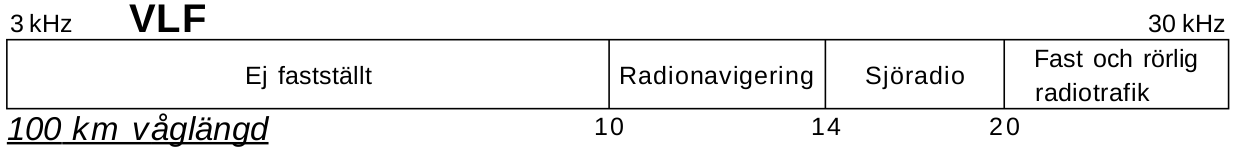
\includegraphics[width=\columnwidth]{blabok/pictures/r6-1-vlf}

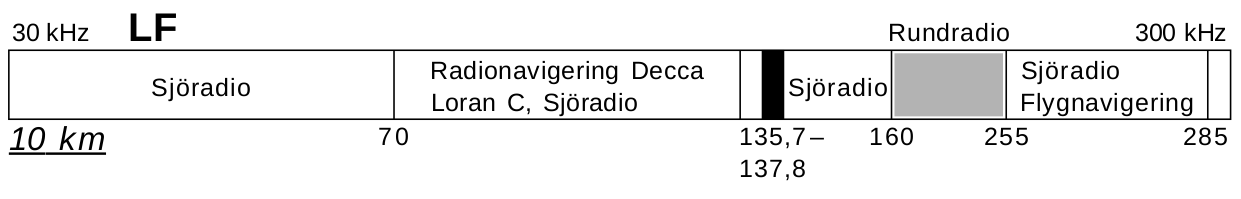
\includegraphics[width=\columnwidth]{blabok/pictures/r6-2-lf}

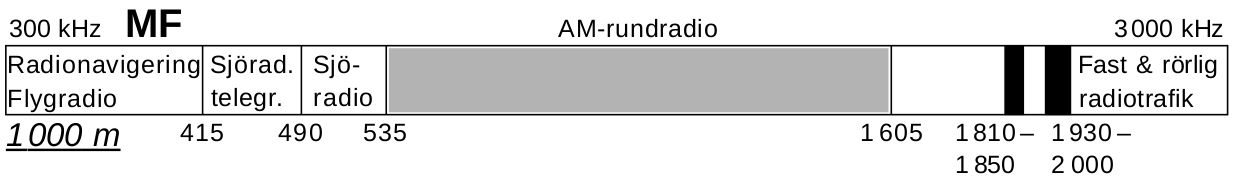
\includegraphics[width=\columnwidth]{blabok/pictures/r6-3-mf}

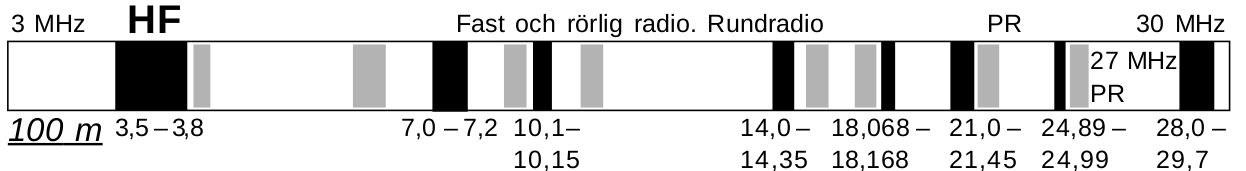
\includegraphics[width=\columnwidth]{blabok/pictures/r6-4-hf}

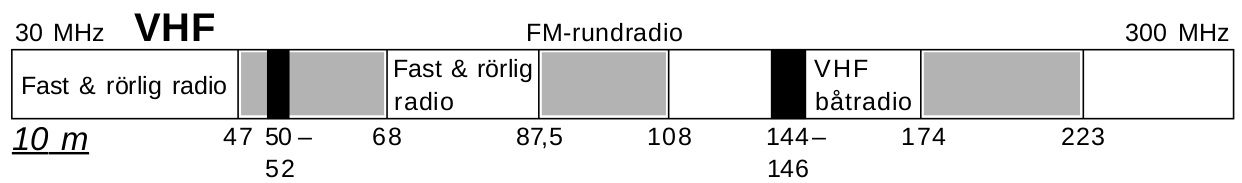
\includegraphics[width=\columnwidth]{blabok/pictures/r6-5-vhf}

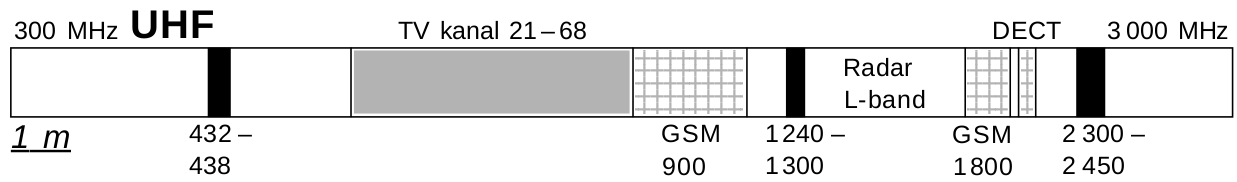
\includegraphics[width=\columnwidth]{blabok/pictures/r6-6-uhf}

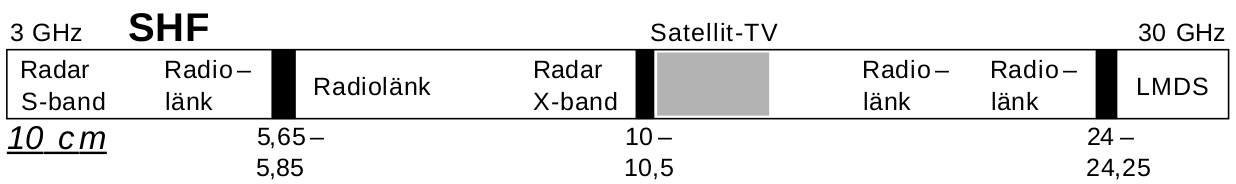
\includegraphics[width=\columnwidth]{blabok/pictures/r6-7-shf}

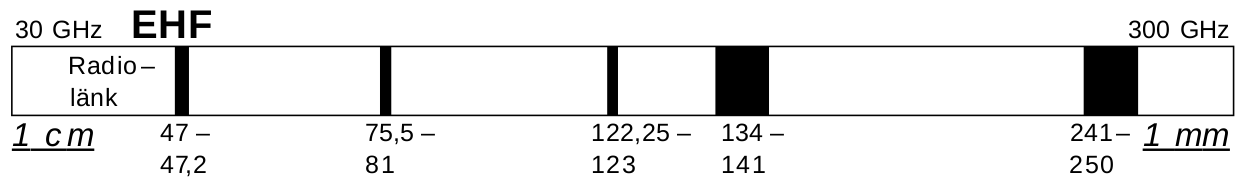
\includegraphics[width=\columnwidth]{blabok/pictures/r6-8-ehf}

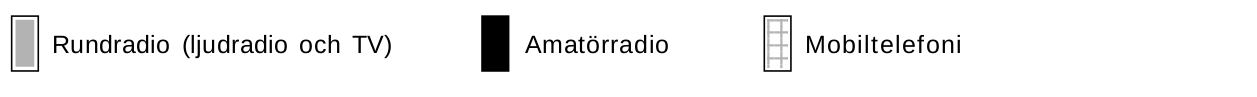
\includegraphics[width=\columnwidth]{blabok/pictures/r6-9}

IARU i region 1 har gjort en detaljerad överenskommelse om hur amatörradiospektrat skall utnyttjas på bästa sätt. Detaljerade bandplaner finns att ladda hem från webbsidan ssa.se där de är översatta till sverige.

Dessa frekvensplaner uppdateras ibland så det är bra att med jämna mellanrum kontrollera om det utkommit ny utgåva och ifall det innebär att man fått ändrade användningsområden på vissa delar.

\section{Repeatertrafik}
	
I många länder finns ett system av relästationer (repeaters) runt de flesta städer.
Dessa relästationer ger dig möjlighet att, med en handapparat eller mobil radioutrustning, ha radiokontakt över ett längre avstånd. Relästationer finns bland annat på 29, 51, 145, 434 och \SI{1297}{MHz}.

Relästationen fungerar så, att det finns en infrekvens och en utfrekvens, som på
t.ex. \SI{145}{MHz} är separerad med \SI{600}{kHz}. Om man vill starta en repeater, sänder man vanligtvis en tonsignal på repeaterns infrekvens. När repeatern startar, sänder den normalt en identifiering på sin utfrekvens. 

\subsection{Bandplan för relätrafik på 29\,MHz}

\begin{tabular}{crr}
	\textbf{Kanal} & \textbf{Din RX} & \textbf{Din TX} \\
	     RH1       &    \num{29,660} &    \num{29,560} \\
	     RH2       &    \num{29,670} &    \num{29,570} \\
	     RH3       &    \num{29,680} &    \num{29,580} \\
	     RH4       &    \num{29,680} &    \num{29,590}
\end{tabular}

\subsection{Bandplan för relätrafik på 50\,MHz}

\begin{tabular}{crr}
	\textbf{Kanal} & \textbf{Din RX} & \textbf{Din TX} \\
	     RF81      &    \num{51,810} &    \num{51,210} \\
	     RF83      &    \num{51,830} &    \num{51,230} \\
	     RF85      &    \num{51,850} &    \num{51,250} \\
	     RF87      &    \num{51,870} &    \num{51,270} \\
	     RF89      &    \num{51,890} &    \num{51,290} \\
	     RF91      &    \num{51,910} &    \num{51,310} \\
	     RF93      &    \num{51,930} &    \num{51,330} \\
	     RF95      &    \num{51,950} &    \num{51,350} \\
	     RF97      &    \num{51,970} &    \num{51,370} \\
	     RF99      &    \num{51,990} &    \num{51,390}
\end{tabular}
	
\subsection{Bandplan för relätrafik på 145\,MHz}

I dag används en kanalindelning om 12,5\,kHz på 145\,MHz medan man tidigare körde 25\,kHz kanalindelning. Jag har valt att även ta med de gamla beteckningarna eftersom de än i dag är vanligare att de används i dagligt tal.

För provet är det dock de nya kanalbenämningarna som man behöver kunna.

\begin{tabular}{llrr}
	\textbf{Kanal} & \textbf{f.d.} & \textbf{Din RX} & \textbf{Din TX} \\
	RV48           & RØ            &        145,6000 &        145,0000 \\
	RV49           & RØX           &        145,6125 &        145,0125 \\
	RV50           & R1            &        145,6250 &        145,0250 \\
	RV51           & R1X           &        145,6375 &        145,0375 \\
	RV52           & R2            &        145,6500 &        145,0500 \\
	RV53           & R2X           &        145,6625 &        145,0625 \\
	RV54           & R3            &        145,6750 &        145,0750 \\
	RV55           & R3X           &        145,6875 &        145,0875 \\
	RV56           & R4            &        145,7000 &        145,1000 \\
	RV57           & R4X           &        145,7125 &        145,1125 \\
	RV58           & R5            &        145,7250 &        145,1250 \\
	RV59           & R5x           &        145,7375 &        145,1375 \\
	RV60           & R6            &        145,7500 &        145,1500 \\
	RV61           & R6X           &        145,7625 &        145,1625 \\
	RV62           & R7            &        145,7750 &        145,1750 \\
	RV63           & R7X           &        145,7875 &        145,1875
\end{tabular}

\chapter{ITU Radioreglemente}
\section{ITU -- Internationella teleunionen}

Vid \emph{internationell} amatörradiotrafik gäller följande reglemente:

\subsection{Utrag ur ITU RR artikel 25}

\begin{tabularx}{\columnwidth}{lX}
	25.1 & Radiokommunikation mellan amatör-
	stationer i olika länder ska vara
	tillåtet, såvida inte administrationen
	i ett av de berörda länderna har
	anmält att de motsätter sig sådan
	radiokommunikation.\vspace{1ex}\\
	
	25.2 & Sändningar mellan amatörstationer
	i olika länder ska vara begränsad till
	kommunikation, som överensstäm-
	mer med ändamålet med amatör-
	radio, enligt definitionen i No. 1.56\footnote{%
		Amatörradiotrafik:
		Icke yrkesmässig radiotrafik för
		övning, kommunikation och tekniska 
		undersökningar, bedriven
		i personligt intresse och utan
		vinningssyfte.}
	och till anmärkningar av personlig
	karaktär.\vspace{1ex}\\
	
	25.2A & Sändningar mellan amatörstationer
	i olika länder ska inte vara kodade
	för att dölja innehållet, utom för
	styrsignaler som utväxlas mellan
	jordkommandostationer och rymd-
	stationer inom amatörradiotjänsten\vspace{1ex}\\
	
	25.3 &Amatörstationer får användas för att
	sända internationell kommunikation
	för tredje part endast vid nödsitua-
	tioner och för katastrofhjälp. En
	administration får bestämma i vilken
	utsträckning detta får tillämpas för
	amatörstationer som omfattas av
	dess regelverk.\vspace{1ex}\\
	
	25.5 &Administrationer ska bestämma
	huruvida en person, som ansöker
	om licens för amatörradio, behöver
	visa färdighet i att sända och ta
	emot texter med morsesignaler.\vspace{1ex}\\
	
	25.6 & Administrationer ska bekräfta de
	operativa och tekniska kvalifikatio-
	nerna hos en person, som ansöker
	om att få använda en amatörradio-
	station.\vspace{1ex}\\



\end{tabularx}	

% Uppdelning av layoutskäl
\begin{tabularx}{\columnwidth}{lX}	
	
	25.7 & Den maximala effekten för en
	amatörradiostation ska anges av de
	aktuella administrationerna.\vspace{1ex}\\
		
	25.9 & Under sändningspassen ska
	amatörradiostationer sända sin
	anropssignal med korta intervall.\vspace{1ex}\\
		
	25.9A & Administrationer uppmuntras att
	vidta nödvändiga steg för att tillåta
	amatörradiostationer att förbereda
	sig för och uppfylla kommunika-
	tionsbehov som stöd för katastrof-
	insatser.\vspace{1ex}\\
	
	25.9B & En administration får bestämma
	huruvida man tillåter en person, som
	erhållit licens för amatörradio av en
	annan administration, att använda
	en amatörradiostation medan per-
	sonen tillfälligt befinner sig på dess
	territorium, med beaktande av de
	villkor eller begränsningar som
	anges.\vspace{1ex}\\
	
	25.10 & Villkoren enligt Sektion I i denna
	artikel ska även gälla, i tillämpliga
	delar, för amatörsatellittjänsten.\vspace{1ex}\\
	
	25.11 & Administrationer som tillåter rymd-
	stationer i amatörsatellittjänsten ska
	försäkra att tillräckligt med jord-
	kommandostationer etableras före
	uppskjutning, för att säkerställa att
	interferens som orsakas av en station
	i amatörsatellittjänsten kan stoppas
	omedelbart.\vspace{1ex}\\
	
\end{tabularx}

\vspace{1em} \hrule \vspace{1em}

\emph{Kom ihåg:}

\begin{itemize}
	\item vid nödsituation och för katastrofhjälp får amatörradion användas i radiotrafik för tredje parts räkning.
\end{itemize}

\emph{Lär dig:}

\begin{itemize}
	\item att sändning mellan amatörstationer i olika länder ska ske på vårdat språk
	\item att under sändningspassen ska amatörradiostationerna sända sina anropssignaler med korta intervaller
\end{itemize}




\chapter{CEPT:s rekommendationer}
CEPT är en samarbetsorganisation av europeiska Post- och Telekommunikationsmyndigheter.

Dess uppgift är att samordna och reglera elektronisk kommunikation inom Europa.
Detta sker genom att ta fram beslut, rekommendationer och rapporter.

För amatörradion finns det två rekommendationer, som kortfattat beskrivs i detta
kapitel.

\section{Rekommendation T/R 61-01}

\textbf{(Turistlicensen)}

CEPT-rekommendationen T/R 61-01
gör det möjligt för sändaramatörer från
CEPT:s medlemsländer att använda amatör-
radiosändare vid temporära besök i andra
CEPT-länder, utan att behöva ansöka om
tillfälligt amatörradiotillstånd.

\emph{\textbf{Anm.} Många länder tillämpar, att turist-
	licensen gäller i högst 3 månader.}

Sedan 1994 finns det också möjlighet för
länder utanför CEPT-sfären att ansluta sig
till denna rekommendation.

\emph\textbf{{Anm.} Vid denna boks tryckning är åtta
	länder anslutna, däribland USA.}

--- TODO: Kontrollera hur det är i dag ---

Det finns endast en licensklass i rekom-
mendationen. Det fordras inte kunskap
i telegrafi, för att få sända på kortvågs-
banden. Några länder kräver dock detta
som ett tillägg.

Varje medlemsland specificerar vilka
nationella licensklasser, som överensstämmer
med CEPT-klassen.

\emph{Alla svenska sändaramatörer är godkända
för CEPT-klassen.}

\section{Utdrag ur tillämpningsföreskrifter}

\begin{tabularx}{\columnwidth}{lX}
3.1 & Sändaramatören ska kunna visa upp
sitt amatörradiotillstånd, eller sitt
amatörradiocertifikat med påtecknad
anropssignal för myndigheten i det
land han/hon besöker.\vspace{1ex}\\
 & \emph{\textbf{Anm.} En notering måste finnas, att
 	rekommendationen T/R 61-01 uppfylls. }\vspace{1ex}\\
 
 3.2 & Det är inte nödvändigt att ta med sig
 sin egen radiostation. Det går också
 bra att låna en station i besökslandet.\vspace{1ex}\\
\end{tabularx}

%För layout
\begin{tabularx}{\columnwidth}{lX}
3.3 & När man sänder i besökslandet ska
CEPT-licensinnehavaren använda sin
nationella anropssignal, föregången av
besökslandets prefix.
Besökslandets prefix och den natio-
nella anropssignalen ska separeras av
tecknet ''/'' (vid telegrafi eller digitala
trafiksätt), eller ordet ”\textbf{streck}”,
engelska ”\textbf{stroke}” eller ”\textbf{slash}” (vid
telefoni).\vspace{1ex}\\

& \emph{\textbf{Anm.} Anropssignalens utformning
i respektive CEPT-land, se tabell på
nästa sida.}\vspace{1ex}\\

3.4 & Att använda CEPT-licensen i ett annat
land, innebär inte några rättigheter att
importera eller exportera radioutrustning, 
utöver de tullbestämmelser som
gäller i respektive land.\vspace{1ex}\\
\end{tabularx}

\emph{Vilka länder, som tillämpar CEPT:s
	rekommendationer T/R 61-01 och deras
	nationella krav och regler, finns i sin
	helhet att läsa på Internet och på SSA:s
	webbplats www.ssa.se under rubriken
	”Att köra radio utomlands”.}

\section{Rekommendation T/R 62-02 harmoniserad certifikatsnivå}

CEPT-licensen enligt Rekommendation
T/R 61-01 kan bara användas vid tillfälligt
besök i annat land.

Om det däremot är en permanent bosättning
kan rekommendation T/R 61-02 användas.
CEPT-länderna har kommit överens om att
samordna kompetenskraven, så att det ska
vara möjligt att erhålla en licens i ett annat
land, utan att avlägga nya prov.

Rekommendationen kallas för HAREC,
Harmonized Amateur Radio Examination
Certificate.

En notering på amatörradiocertifikatet,
att kompetenskraven uppfyller rekommendationen 
T/R 61-02, måste dock finnas.

I kapitel R5 - Anropssignaler 
beskrivs exempel på olika länders
identitetsprefix.

I detta kapitel beskrivs exempel på olika
länders prefix, som sätts före den egna
anropssignalen, vid gästbesök i respektive 
land. Detta prefix kan se annorlunda
ut, jämfört med landets identitetsprefix.

Vilka länder, som tillämpar CEPT:s
rekommendationer T/R 61-02, finns i sin
helhet att läsa på Internet och på SSA:s
webbplats www.ssa.se under rubriken
”Att köra radio utomlands”.

\section{Utdrag ur tabell T/R 61-01}

Prefix som skall användas \textit{före} egen signal vid besök utomlands

\begin{tabular}{ll}
	\textbf{CEPT-land} & \textbf{Prefix} \\
	Belgien            &  ON/\\
	Cypern             &  5B/\\
	Danmark            &  OZ/\\
	England            &  M/\\
	Finland            &  OH/\\
	Frankrike          &  F/\\
	Nederländerna      &  PA/\\
	Irland             &  EI/\\
	Italien            &  I/\\
	Norge              &  LA/\\
	Portugal           &  CT/\\
	Schweiz            &  HB9/\\
	Spanien            &  EA/, EB/\\
	Sverige            &  SM, SA/\\
	Tjeckien           &  OK/\\
	Turkiet            &  TA/\\
	Tyskland           &  DL/\\
	Åland              &  OHØ/\\
	Österrike          &  OE/
\end{tabular}

%\vspace{1em} \hrule \vspace{1em}
% Bara för layout
\newpage

\emph{Kom ihåg:}

\begin{itemize}
	\item Sändaramatörer från CEPT:s medlemsländer har möjlighet att använda
	amatörradiosändare vid temporära besök i annat CEPT-land
	
	\item Sändaramatör ska kunna visa upp sitt amatörradiotillstånd eller
	sitt amatörradiocertifikat i besöks	landet
	
	\item CEPT-licensen ger ingen rätt att importera eller exportera radiout-
	rustning
\end{itemize}


\emph{Lär dig:}

\begin{itemize}
	\item hur olika lönders CEPT-prefix ser ut
	\item att besökslandets prefix skall föregå din anropssignal
\end{itemize}



\chapter{Lagar}
\section{Lagar, föreskrifter och direktiv}

I detta kapitel får du kännedom om lager, föreskrifter och direktiv som reglerar amatörradiotrafik. Det finns inga särskilda lagar eller föreskrifter för amatörradiotrafik.

\subsection{Aktuella lagar}

--- TODO: Kolla relevans och uppdateringar ---

\begin{itemize}
	\item Lagen om elektronisk kommunikation (LEK 2003:389).
	
	\item Yttrandefrihetsgrundlagen, YGL, (1991:1469).
	
	\item Radioutrustningslagen (SFS 2016:392) samt Radioutrustningsförordningen (SFS 2016:394).
	
\end{itemize}

\subsection{Aktuella direktiv}

\begin{itemize}
	\item EMC-direktivet (2014/30/EU) för elektromagnetisk kompatibilitet.
	
	\item Radioutrustningsdirektivet, RED (2014/53/EU), ersätter det tidigare R\&TTY-direktivet.
\end{itemize}

\subsection{Aktuella föreskrifter}

\begin{itemize}
	\item Post- och telestyrelsens föreskrifter om undantag för tillståndsplikt för vissa radiosändare (PTSFS 2018:3).
	
	\item PTS Föreskrift om radioutrustning (PTSFS 2016:5).
\end{itemize}

\section{Vad som regleras?}

\subsection{Lag om elektronisk kommunikation}

Denna lag utgör underlag för de föreskrifter som Post- och telestyrelsen utfärdar för
amatörradiotrafik. Dessutom reglerar lagen vad som gäller vid avlyssning.

Lagen säger att det är tillåtet att avlyssna
ett radiomeddelande, som inte är avsett för
allmänheten, eller ett QSO, men det är förbjudet att föra innehållet i meddelandet vidare.
I lagen finns också straffbestämmelser som bestämmer straffet, om en sändare använ-
des i strid med ett tillståndsvillkor, eller för vidarebefordran av ett avlyssnat medde-
lande.

Om en radiosändare används i brottslig verksamhet, kan denna förklaras förverkad.

\subsection{Yttrandefrihetsgrundlagen YGL}

YGL är en grundlag, som bl.a. reglerar varje
medborgares rätt att i radio och TV offentligen uttrycka tankar, åsikter och känslor.
Det finns också straffbestämmelser i lagenvarför du måste vara försiktig med att inte
förtala, misskreditera, sprida rykten etc.

\subsection{Lag om radio- och teleterminalutrustning}

All kommersiell radioutrustning inkl.
amatörradioutrustningar som säljs ska uppfylla de krav som finns i denna lag.
Det är tillverkarna som ansvarar för att provning sker, enligt fastställda normer.
Amatörradioutrustningar är undantagna från kraven i denna lag, om det rör sig om
byggsatser med lösa delar, eller modifiering av kommersiell utrustning. Detta undantag
möjliggör för en radioamatör att utföra tekniska experiment, utan att behöva köpa
kommersiell utrustning.

\subsection{EMC-direktivet}
Detta direktiv ställer krav på en elektronisk utrustning, att dels inte generera störande radiostrålning, dels kunna motstå störningar från omgivande utrustningar. En kommersiell utrustning som säljs ska vara provad enligt fastställda normer. Uppfylls kraven, ska tillverkaren märka utrustningen med CE-symbolen.

Även i detta direktiv är amatörradioutrustningar som byggs av lösa delar, eller
modifiering av kommersiella produkter undantagna.

\section{Post- och telestyrelsens föreskrifter
	om undantag från tillståndsplikten
	för vissa radiosändare}

Det finns ingen särskild föreskrift för
amatörradiotrafik. Post- och telestyrelsen
har valt att samla all användning av radio-
sändare, som inte kräver tillståndsplikt, i en
enda föreskrift PTSFS 2018:3.

Nedan finns utdrag ur denna föreskrift,
som reglerar kraven för amatörradiotrafik:

\subsection{2 kap. Definitioner}

\begin{tabularx}{\columnwidth}{lX}
	1 § & I dessa föreskrifter avses med
	\textit{amatörradiocertifikat}: kunskapsbevis utfärdat eller godkänt av Post- och telestyrelsen, som utvisar att godkänt kunskapsprov avlagts,
	amatörradiosändare: radiosändare som är avsedd att användas av personer
	som har amatörradiocertifikat, för sändning på frekvenser som är avsedda för
	amatörradiotrafik, \textit{amatörradiotrafik}: icke yrkesmässig radiotrafik för övning, kommunikation
	och tekniska undersökningar, bedriven i personligt radiotekniskt intresse och utan
	vinstsyfte,\vspace{1ex}\\
\end{tabularx}

\subsection{3 kap. Bestämmelser om undantag från tillståndsplikt}

Nedan en tabell över tillåtna effekter. Metod är hur effekten mäts där pep = peak envelope power vid sändarens utgång, erp = utstrålad effekt jämförd med en dipol (0 dBd) och eirp är ekvivalent isotrop effekt jämförd med en tänkt antenn som strålar lika i alla riktningar (0 dBi).

För att få sända mer än 200\,W krävs sedan 1 nov. 2018 ett särskilt tillstånd som kan sökas från PTS. De frekvensband som då påverkas anges i kolumnen ''Tillst.''

\begin{tabular}{rrlr}
	\textbf{Frekvensband} & \textbf{Effekt} & \textbf{Metod} & \textbf{Tillst.} \\
	    137,7--137,8\,kHz &            1\,W & erp            &  \\
	        472--479\,kHz &            1\,W & eirp           &  \\
	      1810--1850\,kHz &          200\,W & pep            &            1\,kW \\
	      1850--1900\,kHz &           10\,W & pep            &  \\
	      1900--1950\,kHz &          100\,W & pep            &  \\
	      1950--2000\,kHz &           10\,W & pep            &  \\
	      3500--3800\,kHz &          200\,W & pep            &            1\,kW \\
	  5351,5--5366,5\,kHz &           15\,W & eirp           &  \\
	      7000--7200\,kHz &          200\,W & pep            &            1\,kW \\
	10\,100--10\,150\,kHz &          150\,W & pep            &  \\
	14\,000--14\,350\,kHz &          200\,W & pep            &            1\,kW \\
	18\,068--18\,168\,kHz &          200\,W & pep            &            1\,kW \\
	21\,000--21\,450\,kHz &          200\,W & pep            &            1\,kW \\
	24\,890--24\,990\,kHz &          200\,W & pep            &            1\,kW \\
	28\,000--29\,700\,kHz &          200\,W & pep            &            1\,kW \\
	      50,0--52,0\,MHz &          200\,W & pep            &  \\
	    144,0--146,0\,MHz &          200\,W & pep            &            1\,kW \\
	    432,0--438,0\,MHz &          200\,W & pep            &            1\,kW \\
	      1240--1300\,MHz &          200\,W & pep            &            1\,kW \\
	      2400--2450\,MHz &         100\,mW & pep            &  \\
	      5,65--5,85\,GHz &          200\,W & pep            &            1\,kW \\
	      10,0--10,5\,GHz &          200\,W & pep            &            1\,kW \\
	   24,00--24,25\,GMHz &          200\,W & pep            &            1\,kW \\
	      47,0--47,2\,GHz &          200\,W & pep            &            1\,kW \\
	       75,5-81,0\,GHz &          200\,W & pep            &            1\,kW \\
	  122,25--123,00\,GHz &          200\,W & pep            &            1\,kW \\
	        134--141\,GHz &          200\,W & pep            &            1\,kW \\
	        241--250\,GHz &          200\,W & pep            &            1\,kW
\end{tabular}

\begin{tabularx}{\columnwidth}{lX}
	14 § & Den som använder en amatörradiosändare ska ha ett amatörradiocertifikat.
	För att få ett amatörradiocertifikat krävs kunskaper i enlighet med Annex 6 i
	CEPT Rekommendation T/R 61-02, Examinering för amatörradiocertifikat, Vilnius 2004, version 5 februari 2016. Undantag från kravet på amatörradiocertifikat gäller för den som under en tidsbegränsad period utbildar sig för att få ett
	sådant certifikat och för den som under en förevisning tillfälligt använder amatörradiosändare, under förutsättning att användningen av radiosändaren sker under
	uppsikt av en innehavare av amatörradiocertifikat.\vspace{1ex}\\
	
	&Den som innehar amatörradiocertifikat ska ha en egen anropssignal. Denna
	framgår av certifikatet, eller tidigare av amatörradiotillståndet. Mottagare- och
	sändarstationens anropssignaler ska sändas i början och i slutet av varje radioförbindelse. Anropssignalerna ska också upprepas med korta mellanrum under
	pågående radioförbindelse. Under de utbildnings- och förevisningstillfällen som
	anges i stycket ovan ska anropssignal användas som tillhör den innehavare av
	amatörradiocertifikat som har uppsikt över användningen av radiosändaren. Vid
	dessa tillfällen får även anropssignal som tillhör den amatörradioförening eller
	institution som anordnar utbildnings- eller förevisningstillfället användas om
	företrädare för föreningen eller institutionen har uppsikt över användningen av
	radiosändaren.\vspace{1ex}\\
	
	&Automatiska amatörradiosändare, till exempel en radiofyr, repeater eller sändare för positionering ska alltid kunna identifieras genom att en anropssignal
	regelbundet sänds med morsetelegrafi, röstmeddelande eller på annat sätt.
	Anropssignalen ska ange vem som är ansvarig för den automatiska sändaren. Den
	som startar eller använder automatiska amatörradiosändare ska ha eget amatörradiocertifikat och ska använda egen anropssignal. Sådan start och användning får
	även utföras av den som inte har amatörradiocertifikat, om det sker under uppsikt
	av en innehavare av amatörradiocertifikat och dennes anropssignal används. 
	\vspace{1ex}\\
\end{tabularx}



\chapter{Dagbok (Loggbok)}
Det finns i dag inget krav på att en radioamatör skall föra loggbok på sina förbindelser. Det finns ändå flera goda skäl till att föra en loggbok när du använder din sändare. 

\section{Radiostörningar}

Genom att föra en loggbok så kan du kontrollea om du har sänt vid tidpunkter som t.ex. grannar har haft störningar på sin utrustning. Detta kan vara viktigt för grannsämjan, särskilt som många kan se med viss skepsis på antenner som sätts upp av sändaramatören.

\section{Vågutbredningsfenomen}

Konditionerna på de olika frekvensbanden varierar och går i olika cykler. Genom att se tillbaka i loggboken kan man bilda sig en uppfattning om vilka tider på dygnet, året och med tiden i solcykeln vilka frekvensband lämpar sig bäst från din plats att nå andra platser.

\section{QSL-kort}

Sändaramatörer skickar QSL-kort (kvittenskort) som bekräftelser på en radiokontakt. Din loggbok är förstås grundmaterialet för att kontrollera inkommande och skicka ut sådana kvittenser.

I dag körs ofta detta digitalt med dator, exempelvis via tjänster som eQSL eller LoTW (loggbook of the world, ARRL:s loggsystem).

\section{Diplom och tävlingar}

För att kvalificera sig i olika tävlingar eller för vissa diplom behöver man kunna styra sina kontakter genom loggböcker och kanske QSL-kort. 

ARRL, den amerikanska amatörradioorganisationen, utger bl.a. DXCC-diplomet,
där kravet är att ha QSL-kort från minst 100 olika radioländer (DXCC-områden).
Amatörradioföreningar eller radioklubbar anordnar även tävlingar (contests). Det går
ut på, att under en bestämd tidsperiod, ha kontakt med så många sändaramatörer som
möjligt. Tävlingstiden kan variera från en timme till flera timmar, ett dygn, eller till och med 48 timmar. Tävlingarna pågår normalt under helgerna. Underlaget för diplomen och tävlingarna utgörs av QSL-korten, eller ibland endast utdrag ur din loggbok.

I dag sköts också detta digitalt via LoTW eller liknande.

Vid tävlingar skickar man in en särskild tävlingslogg. För olika tävlingar gäller lite olika regler för format och hur den skall skickas in. För att få poäng i tävlingarna korsrefereras sedan loggarna så att man ser att de stationer du pratat med också har dig i sina loggar.

\section{Loggens beståndsdelar}

Det finns färdiga loggblad man kan köpa från SSA, man kan också göra egna och skriva ut, färdiga PDF-filer kan enkelt finnas på nätet.

\begin{itemize}
	\item Datum och klockslag i UTC
	\item Motstationens anropssignal
	\item Mottagen och skickad signalrapport (RS/RST)
	\item Frekvensband
	\item Sändningsslag
	\item Den egna effekten
	\item Motstationens namn, QTH, ev. lokatorkoder m.m.
	\item Kommentarer
\end{itemize}

\section{Dataloggning}

Det finns många olika loggprogram för
persondatorer. Många är helt kostnadsfria
och kan hämtas på Internet. Samtliga loggprogram har de uppgifter, som bör finnas med
i dagboken.

De flesta loggprogram har oftast en mängd
funktioner, utöver att vara loggbok. Det finns
t.ex. funktioner, för att styra inställningar av
radiostationen och för att sända och ta emot
telegrafi eller digitala trafiksätt.

\section{Rapportkod (RST-koden)}
Sändaramatörer använder RST-koden, för
att ange hur motstationen hörs.

\begin{itemize}
	\item R står för läsbarhet (readability) och
	graderas från 1 till 5 där 1 är oläsligt och 5 fullt läsbart
	\item S står för signalstyrka (signal strength)
	och graderas från 1 till 9 där 1 är lägst och 9 högst
	\item T står för tonkvalitet (tone) och graderas
	från 1 till 9 där 1 är riktigt dåligt och 9 mycket bra
\end{itemize}

Vid en telefoniförbindelse anges endast
läsbarhet och signalstyrka.

\subsection{R-skalan}

\subsection{S-skalan}

\subsection{T-skalan}



\end{document}
